%% LaTeX2e class for seminar theses
%% sections/content.tex
%% 
%% Karlsruhe Institute of Technology
%% Institute for Program Structures and Data Organization
%% Chair for Software Design and Quality (SDQ)
%%
%% Dr.-Ing. Erik Burger
%% burger@kit.edu
%%
%% Version 1.0, 2018-04-16

\section{Introduction}
\label{ch:Introduction}

The custom ROM scene, especially for older devices is growing continuously. In times, where security vulnerabilities are discovered on a daily basis, software updates are highly important. Due to planned obsolescence and the lack of intrests from OEMs many Android devices are highly outdated and exploitable by most of the common security flaws.

For example, the 2014 \gls{gls:z3}'s last update of Android 6.0 included Security Patches from early 2016, which is already above the common standards on devices released in that timeframe.
\defcitealias{web:dirtycow}{Dirty Cow}
However, that still leaves the device with vulnerabilities like \citetalias{web:dirtycow}, a fairly high security risk.

In order to circumvent this, and thanks to Android being Open Source users can install aftermarket firmware on their device, the so called custom ROM\footnote{The Term ROM originates from old devices that used to have a Read Only Memory for their system partition}. Hence it's possible to always have the latest Security Patches on an fairly old phone. This can't be said about even some of the most recent devices. For example, the \gls{gls:s9} just recently got the Update to Android 9 near Christmas of December 2018\footnote{https://www.netzwelt.de/samsung-galaxy-s9/168265-galaxy-s9-plus-stand-android-90-pie-rollouts-ueberblick.html} whereas, thanks to custom ROMs, the \acrshort{ac:z3} got Android 9.0 back in the end of October, and currently runs the (as per time of writing) 3 days ago released January Security Patches\footnote{\label{jan_asb}https://source.android.com/security/bulletin/2019-01-01} as shown in Figure~\ref{fig:z3_january_asb} below.

\newpage

\begin{figure}
\centering
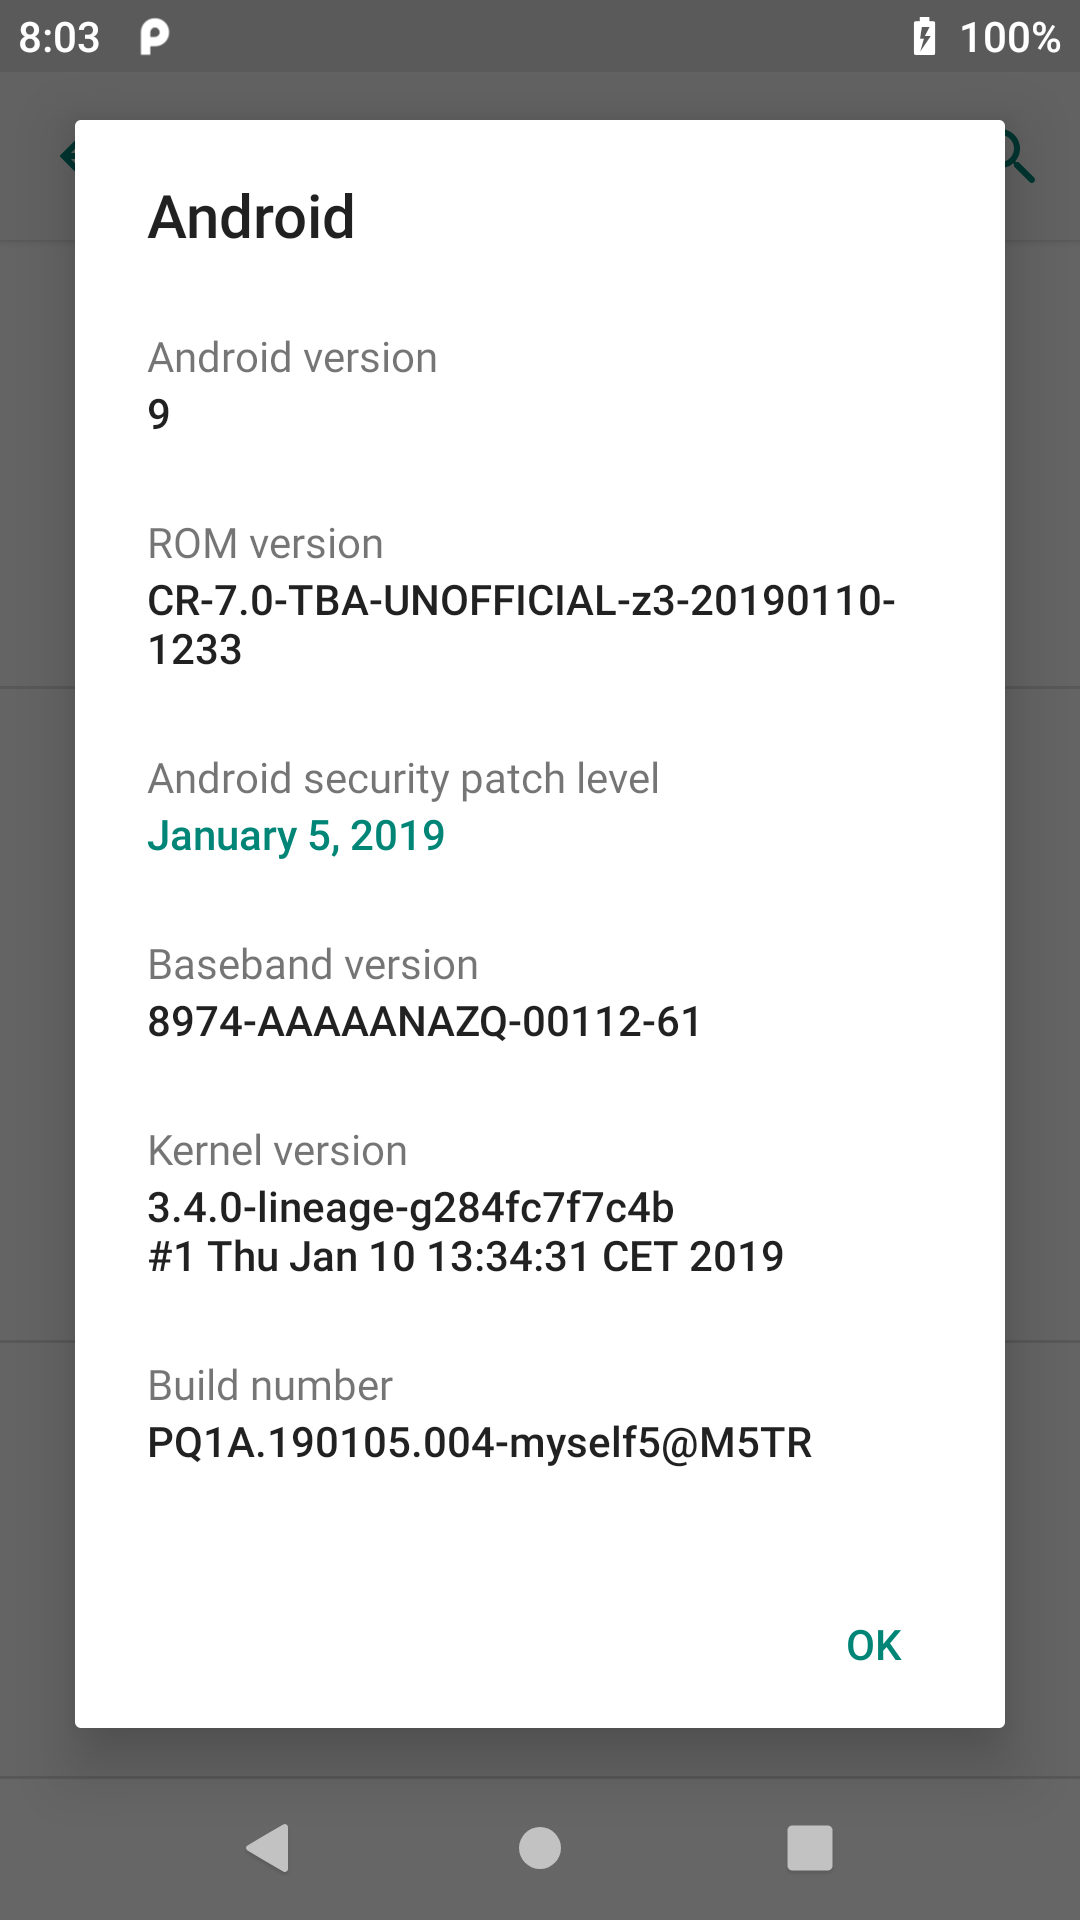
\includegraphics[width=7cm]{images/z3_january_asb}
\caption{\gls{gls:z3} running ~Android 9 with January Security Patches}
\label{fig:z3_january_asb}
\end{figure}

On top of that, the variety of custom ROMs available allows an user to choose between different system sided features that might not be part of the original firmware, which, besides the security patches, is a reason to go custom for many.
In order to provide these aftermarket firmwares each device requires it's own sources, which in addition require certain updates every Major Android revision. These will be explained in detail on the example of the \gls{gls:z3} on \gls{gls:carbon}.
